\documentclass[tikz,border=10pt]{standalone}

\begin{document}
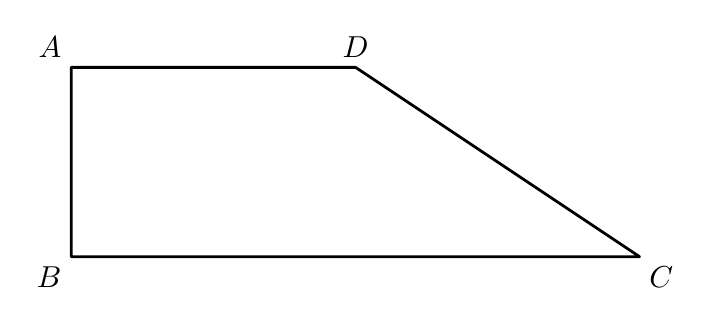
\begin{tikzpicture}[line join=round]
\coordinate (A) at (-3.619,1.208);
\coordinate (B) at (-3.619,-1.196);
\coordinate (C) at (3.599,-1.196);
\coordinate (D) at (-0.006,1.208);

  
  \draw[solid, line width=1.0pt] (A) -- (B) -- (C) -- (D) -- cycle;

  
  \node[above left,  font=\fontsize{10.5}{12.6}\selectfont] at (A) {$A$};
  \node[below left,  font=\fontsize{10.5}{12.6}\selectfont] at (B) {$B$};
  \node[below right, font=\fontsize{10.5}{12.6}\selectfont] at (C) {$C$};
  \node[above,       font=\fontsize{10.5}{12.6}\selectfont] at (D) {$D$};
\end{tikzpicture}
\end{document}